\documentclass{article}
\usepackage{ctex}
\usepackage{geometry}
\geometry{top = 2cm, left = 1cm, right = 1cm, bottom = 2cm}
\usepackage{amsmath,amssymb,amsthm,amsfonts}
\usepackage{abstract}
\usepackage{siunitx}
\usepackage{graphicx}
\usepackage{booktabs}
\usepackage{appendix}
\usepackage{hyperref}
\usepackage{lscape}
\usepackage{multirow}
\usepackage{tikz}

\renewcommand{\appendixpagename}{附录}


\title{用$^{1}\text{H}( ^{19}\text{F}, ^{16}\text{O}^* )\alpha$反应分析氢分布}
\author{钱思天 2001112187}
\begin{document}
    \maketitle
    \begin{abstract}
        氢存在与空气中。在常温下,氢就可以扩散到大多数金属中,
使金属的各种性能发生变化。
长期以来,用常规方法很难分析样品中的氢分布状况。加速器
技术和重离子核反应技术的发展和应用,使无损分析样品中的不同
深度处氢的分布状况成为可能。由于入射粒子只与靶样品中的氢发
生共振核反应,靶样品中其它元素对氢含量分析没有影响,因此这
种方法灵敏度高,也比较准确。本实验利用了2*1.7MV加速器,通过测量$^{19}\text{F}$$^{1}\text{H}( ^{19}\text{F}, ^{16}\text{O}^* )\alpha$的共振核反应放出的光子,测量了样品中混有的氢杂质的分布。
        \newline
        \newline
        {\emph{ 关键词:\ 核反应、2*1.7MV加速器、氢分布 }\rm}

    \end{abstract}

\section{实验原理}
氢存在与空气中。在常温下,氢就可以扩散到大多数金属中,
使金属的各种性能发生变化;例如钢中含氢导致氢脆现象。其他材
料中氢含量的多少也影响其性能。因此,了解材料中氢的存在和分
布状况,在冶金、矿物、半导体、能源、材料等领域的研究中都很
重要。

长期以来,用常规方法很难分析样品中的氢分布状况。加速器
技术和重离子核反应技术的发展和应用,使无损分析样品中的不同
深度处氢的分布状况成为可能。由于入射粒子只与靶样品中的氢发
生共振核反应,靶样品中其它元素对氢含量分析没有影响,因此这
种方法灵敏度高,也比较准确。
\begin{enumerate}
  \item 共振核反应的选择

  本实验采用$^{1}\text{H}( ^{19}\text{F}, ^{16}\text{O}^* )\alpha$共振核反应来测量氢在样品中的分布。入射粒子$^{19}\text{F}$轰击靶核$^{1}\text{H}$发生核反应,生成处于激发态的$^{20}\text{Ne}$核;它退激后发射$\alpha$粒子和处于激发态的$^{16}\text{O}^*$核,$^{16}\text{O}^*$核退激后回
到基态,同时发射$\gamma$光子。该共振反应的末态粒子有$\alpha$粒子和$\gamma$光
子。由于$\alpha$粒子阻止本领较大,测量必须在真空中进行;因此我们
在实验中只测量$^{16}\text{O}^*$核退激发射的$\gamma$光子产额,以确定样品中氢的
含量。探测$\gamma$光子的探测器可以放在靶室之外。
  
  反应截面随入射粒子能量变化的曲线称为核反应的激发曲线。
对应不同的入射$\text{F}$离子能量,
该核反应有两个主要的共振峰,分别在$6.42\si{MeV}$和$16.44\si{MeV}$。共振
峰的形状可用 Breit-Wigner 公式描述:
\begin{equation}
\sigma(E) = \frac{\sigma_R}{1+\frac{E-E_R}{\Gamma/2}^2}
\end{equation}
式中$\Gamma$为共振峰宽度,$E_R$为共振能量,$\sigma_R$为共振截面。
  
  实验采用$6.42\si{MeV}$的共振$\Gamma=55\si{KeV},\sigma=0.1\si{b}$测量氢分布。$6.42\si{MeV}$的共振核反应产生的$^{16}\text{O}$处于激发态,退激时发出能量
分别为$ 6.13,6.92,7.12\si{MeV} $的$\gamma$光子,如图三所示。这三支$\gamma$光
子的分支比比值为:
\begin{equation}
\begin{aligned}
\gamma_1:\gamma_2:\gamma_3&= 2.8:0.016:0.075\\
&\approx 97\%:0.5\%:2.5\%
\end{aligned}
\end{equation}
因此我们可以忽略$\gamma_2$ 和$\gamma_3$ 的贡献,测量时主要记录能量
$6.13\si{MeV}$ 的$\gamma_2$ 光子。

采用$6.42\si{MeV}$的共振核反应,可以测量较深厚度处的氢分布,
因为相邻共振峰相距较远,不会相互影响。另外,$^{16}\text{O}$退激发出的$\gamma$射线能量较高,本底干扰很小,可以忽略入射离子与除氢以外其它
核子发生核反应所放出的$\gamma$射线的影响。同时,也可以提高束流以
缩短测量时间,而不影响测量精度。但$6.42\si{MeV}$的共振峰有一定的
宽度,因此深度分布的测量精度不是很高,约为$200\text{\AA}$至$300\text{\AA}$。
  
  \item   氢分布分析原理

  入射能量为$E_0$(高于共振能量)的氟离子打到待
  分析的样品上,进入样品后逐渐损失能量。设在深度为$x$处,$\text{F}$离
  子的能量损失了$\Delta E$后变为$E$。
  \begin{enumerate}
  \item 氟离子只在其能量为共振能量$E_R$时,才和样品中所含的
氢发生核反应。入射能量$E_0$($>E_R$)的氟离子在进入样品一定
深度(设为 $x$)后,能量降为$E_R$,这时它和该深度处的氢发生
反应。即
\begin{equation}
E = E_0 -\Delta E \approx E_0 - |\frac{dE}{dx}|\times x = E_R
\end{equation}
因此,发生氢反应的深度$x$为
\begin{equation}
x=\frac{E_0-E_R}{|dE/dx|}
\end{equation}
氟 离 子 束 流 能 量$E_0$和 加 速 器 高 压 的 关 系 为$\text{HV}\times(4+1)\si{MeV}$
设$(dE/dx)$的单位为$(\text{eV/\AA})$,则
\begin{equation}
x(\text{\AA})=\frac{[\text{HV}\times(4+1)-6.42]\times10^{6}\text{(eV)}}{|dE/dx|(\text{eV}/\text{\AA})}
\end{equation}
依次改变加速器束流能量 HV,不同入射能量的氟离子就
和不同深度处的氢发生反应,记录反应后产生的氧激发态退
激$\gamma$光子产额 , 就可以得到样品中的氢分布情况。
\item 含量分析:

如前所述,实验时记录氧激发态发出的 6.13MeV 的$\gamma$光
子,多道谱记数能量区间取为 $3-7$MeV。对应每一个高压(或
氟离子入射能量)的测量点,记数时取确定的束流积分电荷;
也就是每个测量点对应同样数量的入射氟离子。这样,在入
射离子数一定、反应截面一定的条件下,记录到的$\gamma$光子越
多,说明样品中的氢含量越多,即氢含量正比于在上述区间
内记录到的$\gamma$光子数。
假设标准样品中,氢沿深度均匀分布,且氢含量$C_{st}$已知,
测量得到$\gamma$光子记数为$N_{st}$。测量未知样品得到$\gamma$光子记数为
$N$;则待测样品的氢含量为
\begin{equation}
C = C_{st}\times\frac{|dE/dx|_{E=E_R}\times N}{|dE/dx|_{st;E=E_R}\times N_{st}}\times\frac{\rho_{st}}{A_{st}}\times\frac{A}{\rho}
\end{equation}
式中
$dE/dx_{E=E_R}$为粒子能量为$E$时在靶物质中的阻止本领,
$\rho$和$A$分别为物质的密度和原子序数,下标$st$表示标准样品。
  \end{enumerate}
\end{enumerate}
\section{实验介绍}
\subsection{实验操作}
\begin{enumerate}
\item 把样品装在靶盘上,装
进靶室,并抽真空,接好
线。靶室上接好“束流”
线(通束流积分仪)和
“抑制”线,“抑制”
加-270V。使 BGO 探测
器对准靶室窗,并加高
压至 580V-600V(调节
钮读数约 4.0 格)。
\item 测本底,作能量刻度。

在实验室及周围环境中,普遍存在着放射性核素钾 40 和
铊 206 的本底,它们发出的$\gamma$光子具有确定的能量,分别为
1460.7 keV 和 2614.3 keV,可以被我们所用的 BGO 探测器探
测到。
从多道谱上我们可以确定这两个本底峰对应的道数。设能
量-道数是线性关系,则由这两个点可以定出一条直线,这样
就可以进行能量-道数的互相转换。

\item 测量标准样品。

我们用 Maestro 软件作数据获取,用束流积分仪控制记数
的开始和停止(设置:“Services”;->“Job”->“Control”->
“D:User”->“GATEON.JOB”->“OK”)。根据上面本底测
量定出的能量-道数关系,在多道上选取对应$3-7$MeV 的道
数区间,落在该区间的$\gamma$光子将被记数。
我们所用的标准样品中,所含的氢均匀分布在约$2\si{\micro m}$的
非晶硅层,该层是在单晶硅衬底上通过辉光放电沉积而成的。
给定的标准样品中含氢的原子比为 13.9\%。

测量时,每个点束流积分取 $15-20$ 微库,高压从 1.30 开
始取 5 个点,对应样品表面以内 5 个不同深度。5 个点的平均
记数作为标准样品的记数 $N_{st}$ 。在每个测量点,分别记录高压
值、$\gamma$光子在$3-7$MeV 区间内积分记数、测量时间、束流积
分($\si{\micro C}$)和流强($\si{nA}$)。
\item 测量未知含量样品。

未知样品表面大多含氢,可测到一个表面峰。有的样品内
部也有氢分布。测量时从高压 1.26 开始。
 
\end{enumerate}

\section{实验记录与数据处理}
\subsection{刻度}
直接测量环境本底得到的两个峰的测量结果如表\ref{tab:1}。
\begin{table}[htbp]
  \centering
  \caption{利用环境本底进行标定结果\label{tab:1}}
  \begin{tabular}{rrrr}
\toprule
 Degree &  Count &  Degree &  Count \\
\midrule
    -10 &   1400 &       1.0 &  29148.0 \\
     -9 &   3169 &       2.0 &  28206.0 \\
     -8 &   5460 &       3.0 &  26948.0 \\
     -7 &   9434 &       4.0 &  25646.0 \\
     -6 &  12398 &       5.0 &  23441.0 \\
     -5 &  17243 &       6.0 &  21836.0 \\
     -4 &  20354 &       7.0 &  18736.0 \\
     -3 &  24540 &       8.0 &  17042.0 \\
     -2 &  27074 &       9.0 &  13331.0 \\
     -1 &  28412 &      10.0 &  10628.0 \\
      0 &  29291 &       -- &      -- \\
\bottomrule
\end{tabular}

\end{table}

利用测量结果,将$160-350$道作为目标$\gamma$光子的计数区段。
\subsection{标样的测定}
标样的测量结果记录如表\ref{tab:2}。
\begin{table}[htbp]
  \centering
  \caption{标样的测量结果\label{tab:2}}
  \begin{tabular}{rrr}
\toprule
 DegreeOrigin &  DegreeReal &  Count \\
\midrule
           20 &          20 &     81 \\
           25 &          25 &     16 \\
           30 &          30 &      5 \\
           35 &          35 &      1 \\
           40 &          40 &      0 \\
           45 &          45 &   \color{red}{1999} \\
           50 &          50 &   \color{red}{4914} \\
\bottomrule
\end{tabular}

\end{table}
后续会采用标样的平均计数作为标样的计数值。
\subsection{样品10的测量结果}
样品10的测量结果记录如表\ref{tab:3}。
\begin{table}[htbp]
  \centering
  \caption{样品10的测量结果\label{tab:3}}
  \begin{tabular}{rrrr}
\toprule
 HV[MV] &  I[nA] &  t[s] &    N \\
\midrule
   1.26 &   2.85 & 75.48 &   89 \\
   1.30 &   2.85 & 77.82 &  956 \\
   1.34 &   2.90 & 72.42 & 1138 \\
   1.38 &   2.95 & 69.70 & 1078 \\
   1.42 &   2.90 & 72.00 &  750 \\
   1.46 &   2.90 & 71.66 &  282 \\
   1.50 &   2.90 & 71.24 &  116 \\
\bottomrule
\end{tabular}

\end{table}
因为样品10是不锈钢,所以在后面的分析中,采用的成分为:Fe 71\%, Cr 19\%, Ni 10\%,密度为$7.39\si{g\per cm^3}$。
\subsection{氢含量分析}
直接计算,可以得到氢含量的分布表\ref{tab:4}及图\ref{fig:1}。
\begin{table}[htbp]
  \centering
  \caption{不同深度的氢含量计算表\label{tab:4}}
  \begin{tabular}{rrr}
\toprule
 DegreeOrigin &  DegreeReal &  Count \\
\midrule
           22 &          20 &     99 \\
           27 &          25 &     25 \\
           32 &          30 &      6 \\
           37 &          35 &     10 \\
           42 &          40 &      2 \\
           47 &          45 &      9 \\
           52 &          50 &   \color{red}{8956} \\
\bottomrule
\end{tabular}

\end{table}
\begin{figure}
  \centering
  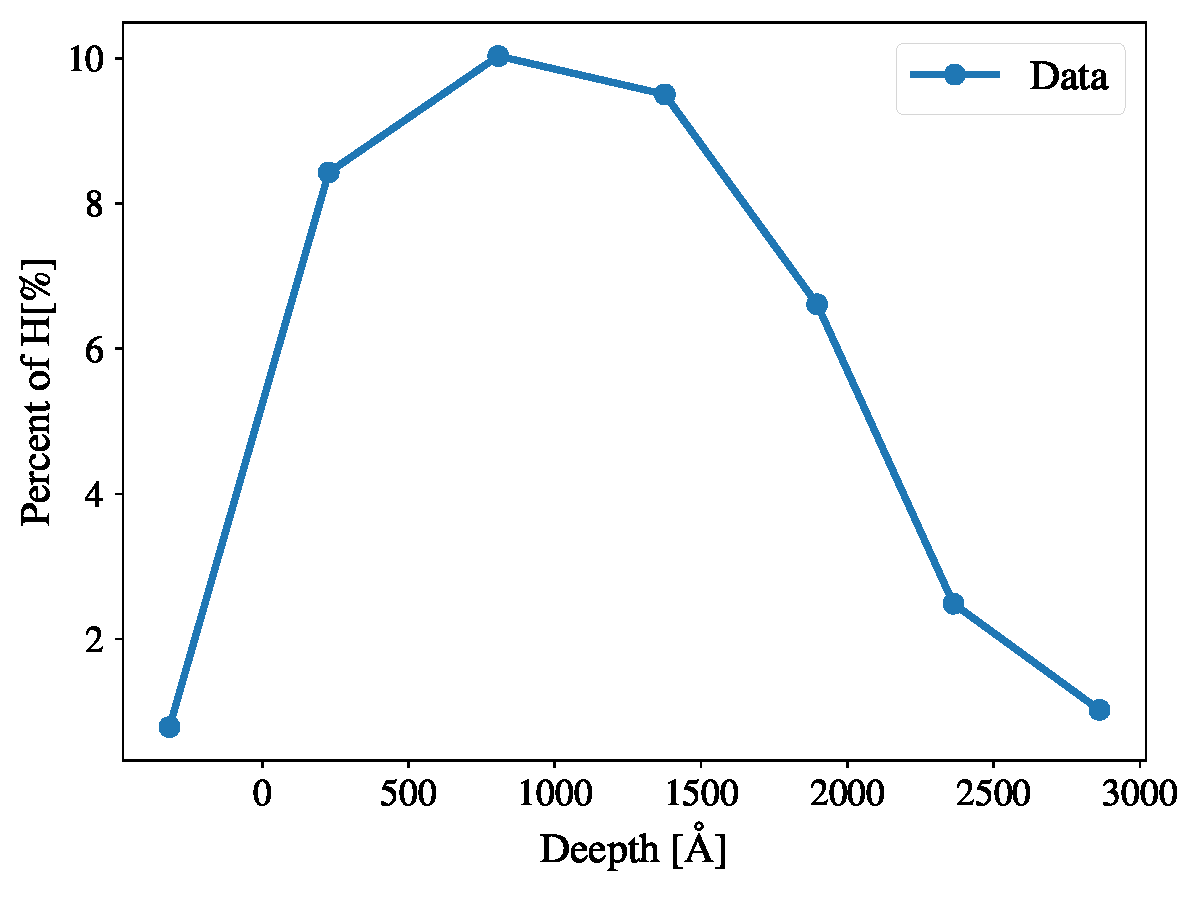
\includegraphics[width=0.7\textwidth]{../Analysis/Hpercent.pdf}
  \caption{不同深度的氢含量计算图\label{fig:1}}
\end{figure}
\section{致谢}
    感谢赵捷老师和徐川老师的帮助和指导。 
\end{document}